\chapter[\hspace{0pt}模型建立与求解]{{\heiti\zihao{3}\hspace{0pt}模型建立与求解}}\label{chapter4: 模型建立与求解}
% \setcounter{page}{4} % 这里要在论文摘要和符号表写完后手动修改页码

\removelofgap
\removelotgap

%% 文章标题架构
% 一级 chapter      : \chapter[\hspace{0pt}模型建立与求解]{{\heiti\zihao{3}\hspace{0pt}模型建立与求解}}\label{chapter4: 模型建立与求解}
% 二级 section      : \section[\hspace{-2pt}问题1:路旅游方案设计]{{\heiti\zihao{-3} \hspace{-8pt}问题1:路旅游方案设计}}\label{section3: 问题1:路旅游方案设计}
% 三级 subsection   : \subsection[\hspace{-2pt}模型建立与求解]{{\heiti\zihao{4} \hspace{-8pt}模型建立与求解}}\label{section3: 模型建立与求解}
% 四级(顶格)        : \noindent\textbf{(1)参数编码与搜索空间}
% 四级(不顶格)      : \textbf{}
% 五级(尽量别用)    : \circled{1} \textbf{$\Delta E_{00}$损失值统计}
% 
%% 公式、图片、表格

% 公式:
% 1. 中间不必加上$$符号
% 2. 在equation后面加上*可以不要自动编号
% \begin{equation}
% \begin{aligned}
%   &u_{i,j}=
%   \begin{cases}
%     v_{i,j}^{(t)},&\text{if } \mathrm{rand}_j\le CR\text{ or } j=j_{rand},\\
%     x_{i,j}^{(t)},&\text{otherwise},
%   \end{cases}
% \end{aligned}
% \end{equation}

% 图片:
% \begin{figure}[h]
% \centering
% \captionsetup{font={small, stretch=1.312}}
% 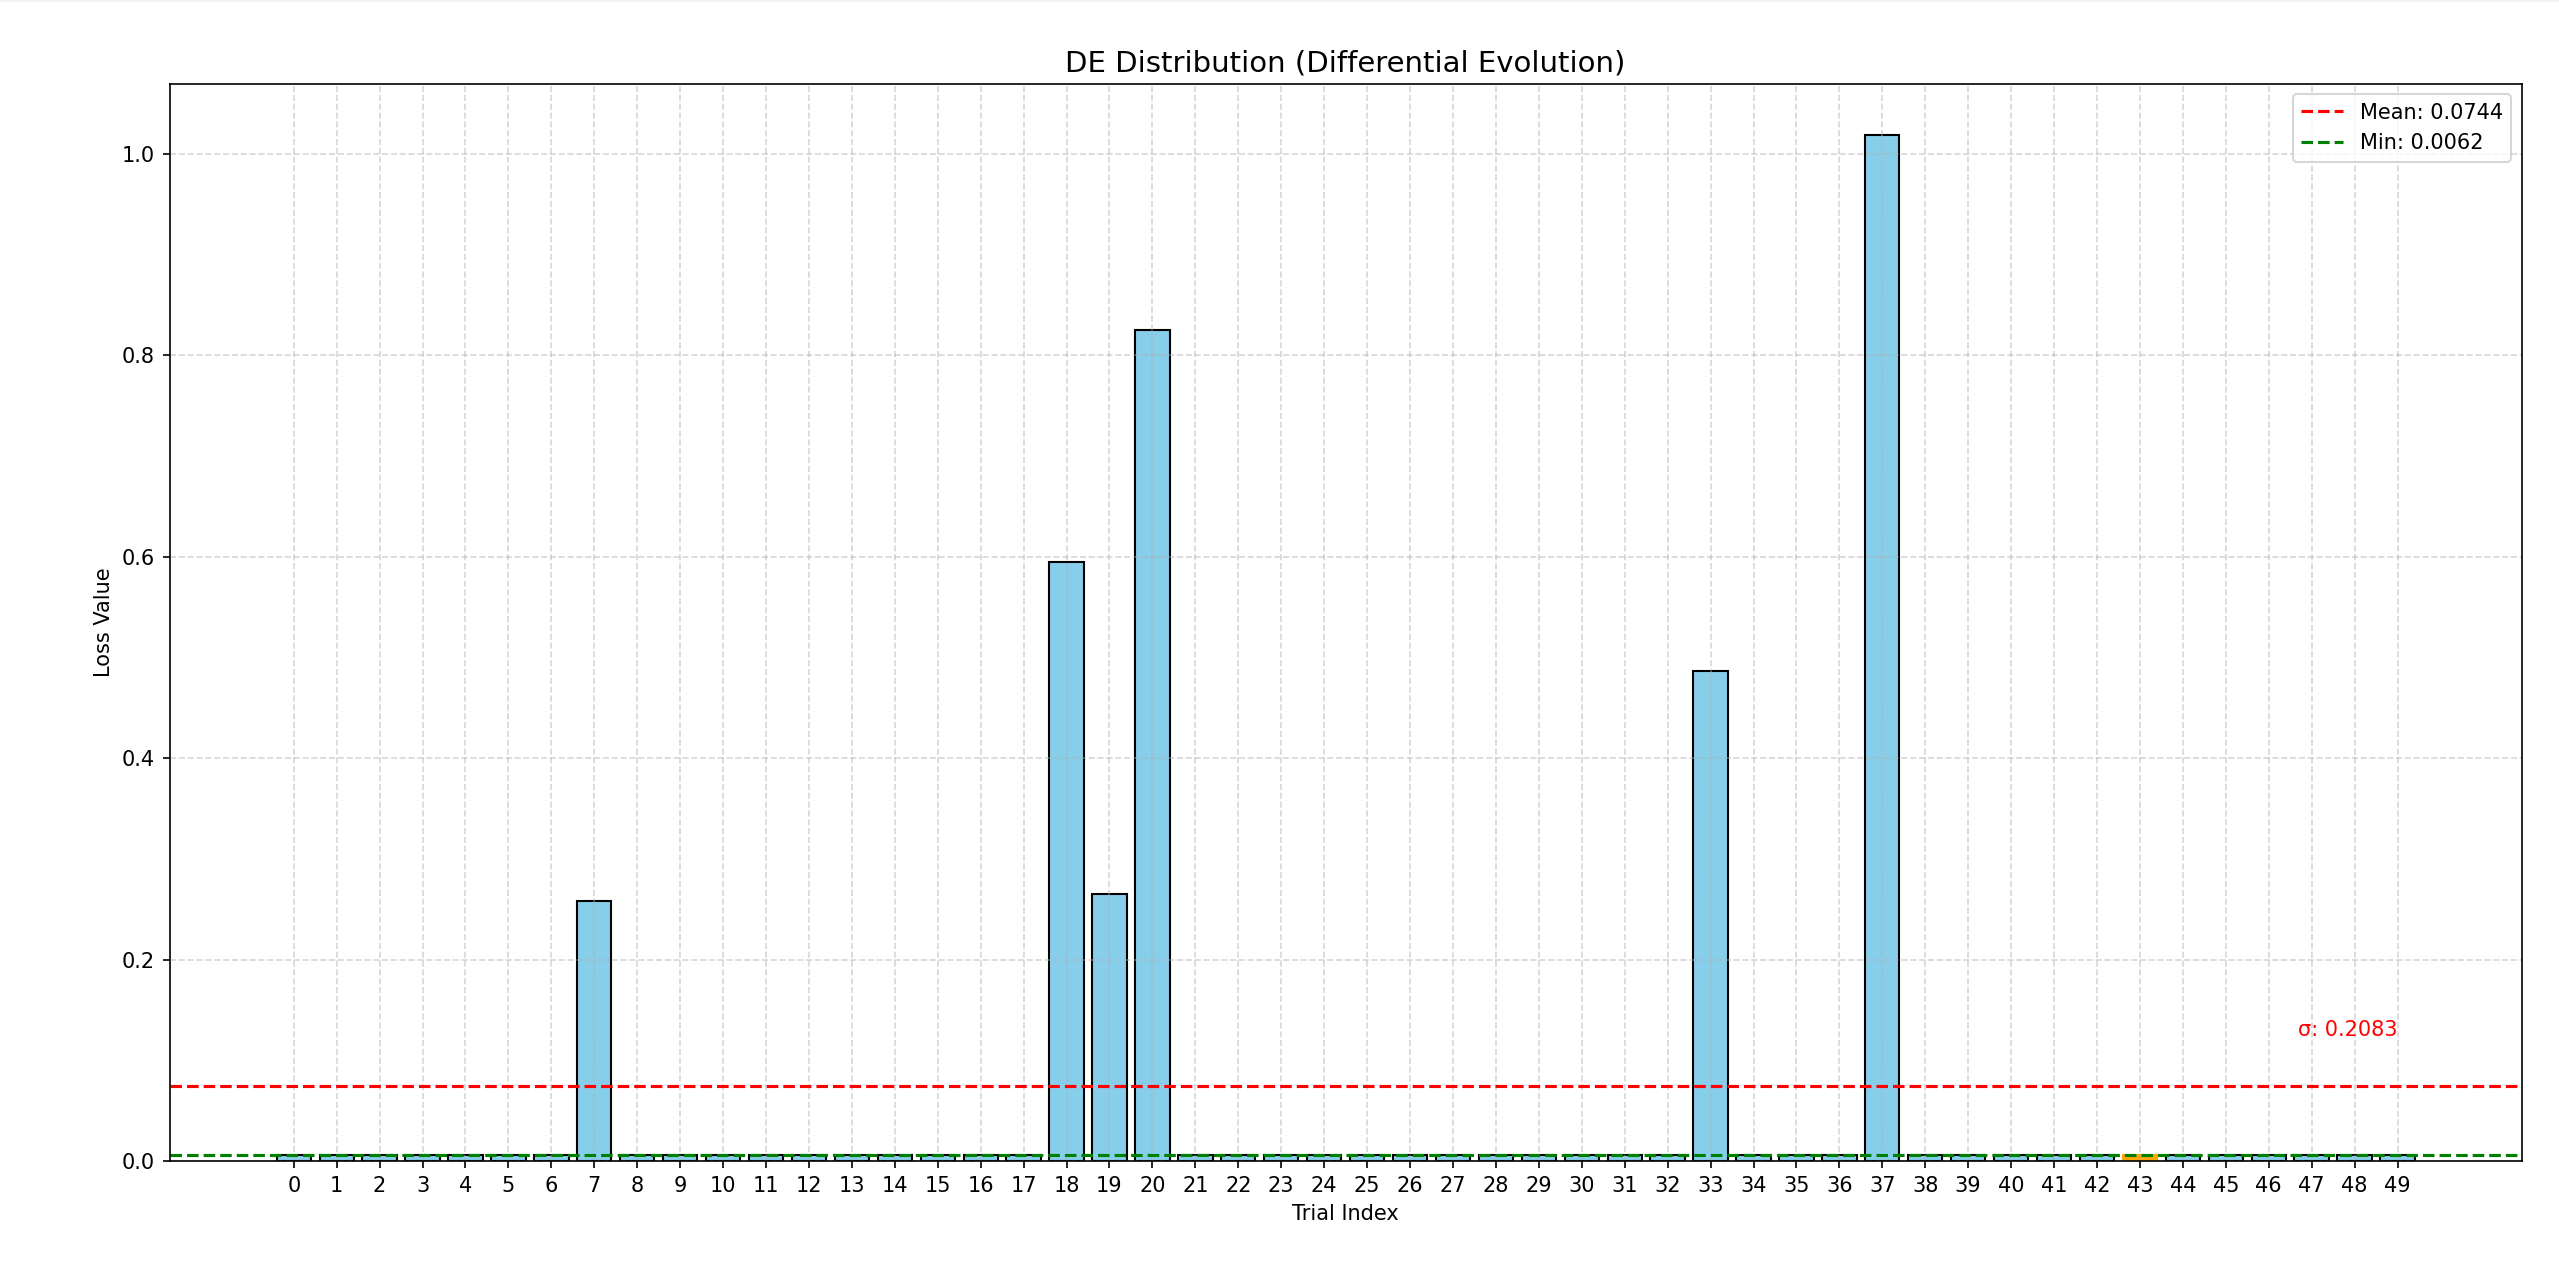
\includegraphics[width=1.0\columnwidth]{figures/DE2000.png}
% \bicaption[50次独立优化实验柱状损失图]{50次独立优化实验柱状损失图。}[Histogram of loss values from 50 independent optimization experiments]{Histogram of loss values from 50 independent optimization experiments.}
% \label{figure3: 柱状loss}
% \end{figure}
% 引用方式:在文字后面加上:\ref{figure3: 柱状loss}

% 表格:
% \begin{table}[h!]
% \small    % 设置表格字体为5号
% \setstretch{1.245}        % 设置具有指定弹力的橡皮长度(原行宽的1.2倍)
% \captionsetup{font={small, stretch=1.512}}
% \centering
%\bicaption[不同基色图像的伽马参数估计结果]{不同基色图像的伽马参数估计结果。}[Gamma parameter estimation results for different primary color images]{Gamma parameter estimation results for different primary color images.}    % 中英文标题


\section[\hspace{-2pt}问题一:路旅游方案设计]{{\heiti\zihao{-3} \hspace{-8pt}问题一:路旅游方案设计}}\label{section3: 问题1:路旅游方案设计}

\subsection[\hspace{-2pt}模型建立与求解]{{\heiti\zihao{4} \hspace{-8pt}模型建立与求解}}\label{section3: 模型建立与求解}

对于此问题,我们首先通过Floyd‑Warshall算法补全邻接矩阵,得到任意两点之间的最短距离。这样我们就可以得到任意区域到任意景点的交通费用和交通时间。以此为基础,我们进行以下建模:

\textbf{景点收益:}由于缺乏具体景点评分数据,我们假设每个景点具有相近的吸引力价值,即此处不加入游客对景点的偏好因素。$P_{max}$表示某一类型的方案的最大满意度(即总是选择游客喜好程度最高的区域3)。

\begin{equation}
  \begin{aligned}
  \text{Pref}^{(d_{p})}_{max}(type)=\begin{cases}
  9\times 1+2=11, & \text{(1日)}\\
  9\times 3+4=31, & \text{(2日)}\\
  9\times 5+6=51, & \text{(3日)}
  \end{cases}
  \end{aligned}
  \end{equation}

以上方程为景区最大收益函数。为了减少数值对模型计算的影响,我们对三种收益进行归一化处理。

\textbf{区域收益:}套餐$p$涉及到的区域的用餐以及住宿体验。根据题目数据,我们将区域喜好度评分$P_{R_{j}}$作为游客在该区域用餐/住宿获得的满意度。如果套餐跨多日,可能涉及多个不同的区域,则将相应区域的偏好分累计。若在同一天中午和晚上都在同一$R_{j}$区域,则游客在该天对区域$R_{j}$的体验包括午餐和晚餐+住宿,为方便建模并突出问题的重心,我们采用叠加的方式计算区域满意度。

\textbf{交通的时间与费用成本:}每套旅游方案中的交通费用和时间开销会降低满意度。我们采用函数$Cost(p)$来评价一个方案中的所有交通费用,用$Time(p)$来表示所有时间开销。此外我们为其增加了权重$w_{\text{cost}}, w_{\text{time}}$,以此代表不同套餐的倾向,用以区分经济优先还是时间优先。

\begin{equation}
\begin{aligned}
  Cost(p) = 
\end{aligned}
\end{equation}

\begin{equation}
  \begin{aligned}
    Time(p) = 
  \end{aligned}
\end{equation}
  



总的某方案$p$的满意度函数如下:

\begin{equation}
\begin{aligned}
  u_p \;=\; w_{\text{pref}}\frac{\text{Pref}(p)}{\text{Pref}_{\max}^{(d_p)}} \;-\; w_{\text{cost}}\frac{\text{Cost}(p)}{\max\{\text{Cost}(q):q\in \mathcal{P}\}} \;-\; w_{\text{time}}\frac{\text{Time}(p)}{\max\{\text{Time}(q):q\in \mathcal{P}\}},
\end{aligned}
\end{equation}

\textbf{最大化函数:}
\begin{equation}
  \begin{aligned}
    Z = \sum_{p\in \mathcal{P}}u_{p}\cdot x_{p}.
  \end{aligned}
\end{equation}

约束条件:
\noindent\textbf{1.景点接待容量限制:}各景点在各个半天时段的接待总人数不得超限。由于早午两段和最多3天行程共有6个半天时段,模型将假设景点容量可在不同时段重复利用。对每个景点 $i\in S$ 有:

\begin{equation}
  \begin{aligned}
    \sum_{p\in \mathcal{P}}\delta_{i,p}\cdot x_{p} \leq 6\,C_{S_{i}},\quad i=1,2\dots ,6,
  \end{aligned}
\end{equation}
其中$\delta_{i,p}=1$当路线$p$包含景点$i$(即游客在某一时段游览了景点$i$),否则$\delta_{i,p}=0$。

\noindent\textbf{2.午餐餐厅容量约束:}每个区域的午餐接待能力(每天中午)也限制了路线分配。类似地,如果认为最多3个中午时段可复用,则对每个区域 $j\in R$:

\begin{equation}
  \begin{aligned}
    \sum_{p\in \mathcal{P}}\theta_{j,p}\cdot x_{p} \leq 3\,L_{R_{j}},\quad j=1,2,\dots ,6,
  \end{aligned}
\end{equation}
其中$theta_{j,p}$代表路线$p$在中午曾安排于区域$j$就餐次数(一日游有1次午餐、三日游有3次午餐机会,但可能某些路线会重复去某一区域)。代码中简化为每个区域午餐总游客$\le C^{\text{lunch}}_j$,相当假定所有行程共用一个中午时段容量,这在行程跨多日的情况下略趋保守。

\noindent\textbf{3.晚餐及住宿容量约束:}每个区域用于晚餐和住宿的容量在不同夜晚也可重复利用。三日游行程最多涉及2晚,故每区域最多2个夜晚可安排住宿。对每个区域 $j\in R$:
\begin{equation}
  \begin{aligned}
    \sum_{p\in \mathcal{P}}\phi_{j,p}\cdot x_p \;\le\; 2\,C^{\text{night}}_j, \quad j=1,\dots,6,
  \end{aligned}
\end{equation}

其中$\phi_{j,p}$为路线$p$在夜晚留宿于区域$j$的次数(二日游路线有1晚、三日游有2晚,一般假定同一线路不重复入住同一酒店区域)。

\noindent\textbf{4.游客总数约束:}根据预期需求,分别规定各类行程分配的总游客数。例如,设定选择一日游的游客总数为$N_{1}$人、二日游$N_{2}$人、三日游$N_{3}$人。则对每一种行程类型分别有:
\begin{equation}
  \begin{aligned}
    \sum_{p\in P_{1\text{day}}}x_p = N_{1},\qquad \sum_{p\in P_{2\text{day}}}x_p = N_{2},\qquad \sum_{p\in P_{3\text{day}}}x_p = N_{3}.    
  \end{aligned}
\end{equation}

代码实现中分别令一日游、二日游总游客数为30,000,三日游为20,000。

约束处理完成后,我们将采用枚举的方式得到一日游、二日游等的所有可能方案。再将其加入到MILP模型中。结合遗传算法选择高质量路线,并采用启发式规则进行路线多样化拓展。最终得到最合适的旅游路线。

\subsection[\hspace{-2pt}问题一结果分析]{{\heiti\zihao{4} \hspace{-8pt}问题一结果分析}}\label{section4: 问题一结果分析}

根据$w_{cost}$TODO,我们可以设置不同权重,得到不同侧重点的旅游方案。本论文设置了三种情况。

\textbf{均衡型:}

\textbf{经济型:}

\textbf{时间节约型:}



\section[\hspace{-2pt}问题二:方案优化]{{\heiti\zihao{-3} \hspace{-8pt}问题二:方案优化}}\label{section3: 问题2:方案优化}

\subsection[\hspace{-2pt}问题分析与建模目标]{{\heiti\zihao{4} \hspace{-8pt}问题分析与建模目标}}\label{section2: 问题分析与建模目标}

当要求旅游套餐种类总数不超过10种时,需要对上述模型进行适应性修改。原模型在追求最大满意度下,可能启用许多不同路线方案来绕开局部容量瓶颈,从而方案种类较多。如果限制套餐类型数$\le10$,模型必须在满意度与管理简化之间折中。我们做出了如下调整:

\noindent\textbf{加入套餐数量约束:}增加约束$\displaystyle\sum_{p\in P}y_p \le 10$,限制被选用的不同路线方案数不超过10种。其中$y_p$为0-1变量,表示方案$p$是否被采用。并引入逻辑约束$x_p \le N_{\text{total}};y_p$(或大$M$法)将$x_p$与$y_p$关联。这样仅当$y_p=1$时,$x_p$可取正值,否则该路线不分配游客。此调整实质上将线性规划扩展为混合整数规划,有助于直接在求解过程中控制方案种类数上限。

\noindent\textbf{精选候选路线集:}在模型求解前预先筛选和精简路线集合$P$,只保留若干“优选”套餐候选。比如,根据单条路线的满意度系数$u_p$对候选方案排序,选取满意度高且覆盖面广的前若干条路线进入优化。原模型生成的路线非常多(一日游$6\times5\times6=180$种,二日游上限$10^4$种,三日游经遗传算法+启发式生成5000种),有许多方案实际贡献的游客数很小甚至为0。我们可剔除明显次优或冗余的方案,例如去除行程过长费用偏高而偏好分较低的组合,或者对行程相似且收益接近的方案只保留其中一种。这相当于在不增加过多成本的前提下人工设定候选集精简至$\le10$条路线,然后在此基础上重新优化分配。这种路线筛选(如按满意度排序取Top 10)和聚类归并的方法可极大减少方案种类,同时尽量保证总满意度接近原最优值。

\noindent\textbf{优先级调度与容量放宽:}在仅允许提供有限几种套餐时,可考虑适当调整对容量约束的处理,确保主要景点和区域得到利用。例如,将重点偏好的景点设计为\**固定线路**,优先占用一定游客量,然后对剩余游客采用次优线路。在代码实现层面,可以对生成的候选路线按照偏好得分或单位满意度收益排序,优先选取少数几条高效路线分配游客直到触及某一容量约束,再引入下一优方案。这种贪心分配过程可以模拟人工规划几种典型套餐的思路:例如优先设计几条涵盖热门景区且总体花费合理的线路,再视剩余接待资源补充其他路线,从而将总套餐数控制在上限之内。

综上,当限制套餐总数不超过10种时,模型需要从“穷尽所有可能组合求全局最优”转变为“在有限方案中求近优”。这要求在模型中增加**组合选择的决策变量和约束**,或采用启发式策略筛选方案。通过上述调整,既能满足管理方便的要求,又尽可能兼顾游客满意度和资源利用的均衡。模型的结构与求解思路具有一定灵活性:无论是通过加入$y_p$变量实现严格的种类约束,还是通过缩减候选路线集来隐含满足要求,都体现了对原优化模型的适应性改进。

\subsection[\hspace{-2pt}模型求解和结果分析]{{\heiti\zihao{4} \hspace{-8pt}模型求解和结果分析}}\label{section2: 模型求解和结果分析}


\section[\hspace{-2pt}问题三:旅馆建设规模与位置选择]{{\heiti\zihao{-3} \hspace{-8pt}问题三:旅馆建设规模与位置选择}}\label{section4: 问题3:旅馆建设规模与位置选择}

\subsection[\hspace{-2pt}模型建立流程]{{\heiti\zihao{4}\hspace{-8pt}模型建立流程}}\label{subsec:3-model-build}


本模型旨在分析重庆旅游景区的住宿扩容问题,基于游客需求、交通成本、时间消耗和景区容量等因素,通过构建优化模型对扩容方案进行评估。

\noindent\textbf{首先,模型采用了基于规模报酬递减的扩容成本函数:}
\begin{equation}
  \begin{aligned}
    C(\Delta K)=c_{1}(\Delta K)^{\gamma}, \quad c_{1} =7\times 10^{-4}\text{(亿元)}, \gamma = 1.09
  \end{aligned}
\end{equation}

此扩容成本函数是采用来自网络的数据统计,并进行处理后得到的。

\noindent\textbf{并定义了经济收益函数 $B(\Delta K)$:}

\begin{equation}
  \begin{aligned}
    B(\Delta K) = v_{s}[Z(K)-Z(K^0)]+v_{p}[N(K)-N(K^{0})]
  \end{aligned}
\end{equation}

其中考虑了扩容后满意度增量和游客接待量的增量。满意度增量通过扩容后游客对旅游线路的偏好变化进行计算,接待量增量则基于实际可接待游客人数与扩容前的差异。

\noindent\textbf{扩容决策的目标是最大化净收益:}

\begin{equation}
  \begin{aligned}
    \underset{r,\Delta K\geq 0}{max}  F_r(\Delta K) = B_r(\Delta K) - C(\Delta K)
  \end{aligned}
\end{equation}

即通过选择最优区域和扩容规模 $\Delta K$,使得总的经济效益最大。模型通过枚举不同区域和容量增量,计算每种方案的经济收益,并结合遗传算法和线性规划(MILP)对扩容后的最优游客分配进行求解。最终,选出净收益最大的扩容方案,并提供详细的扩容规模及其对应的效益曲线。



该模型不仅帮助政府和企业做出最优的扩容决策,还能评估不同扩容方案的经济影响,为旅游业的长期规划提供支持。

\subsection[\hspace{-2pt}模型求解]{{\heiti\zihao{4}\hspace{-8pt}模型求解}}\label{subsec:3-model-build}

模型的求解采用“双层结构”。外层离散搜索扩容区域$r$与规模$\Delta K$,内层维持既有的“枚举路线结合MILP”的流程:

\noindent\textbf{外层:}

\begin{equation}
  \begin{aligned}
    \underset{r,\Delta K \geq 0}{max} F_{r}(\Delta K)
  \end{aligned}
\end{equation}

\noindent\textbf{内层:}
\begin{equation}
  \begin{aligned}
    Z(K),N(K)=arg\quad \underset{x}{max} \sum_{i}s_{i}x_{i}\\
    s.t. \text{容量约束}K
  \end{aligned}
\end{equation}

具体算法如下所示:

\begin{algorithm}[H]\small
  \setstretch{1.245}
  \renewcommand{\algorithmcfname}{算法}
  \caption{旅游景区扩容优化算法}

  \KwIn{原始夜宿容量 $K_0=(K_1^0,\dots,K_6^0)$;扩容步长集合
        $\Delta\mathcal K=\{0,0.5,1,\dots,\Delta K_{\max}\}$;游客需求 $T^0$}
  \KwOut{最优扩容区域 $r^*$、规模 $\Delta K^*$ 及最大净收益 $F^*$}

  \textbf{步骤1:基准求解}\;
  $\text{base\_results}\leftarrow\text{optimizer.run\_optimization}(K_0)$\;
  取 $Z(K^0),\,N(K^0)$\;

  \textbf{步骤2:区域与扩容规模枚举}\;
  \For{$r\leftarrow1$ \KwTo $6$}{
    \For{${\Delta K}\in\Delta\mathcal K$}{
      $K_r \leftarrow K_r^0 + \Delta K$\tcp*{修改容量上限}
      $\text{cur} \leftarrow \text{optimizer.run\_optimization}(K_r)$\;
      取 $Z(K),\,N(K)$\;
      $B = v_s\bigl[Z(K)-Z(K^0)\bigr] + v_p\bigl[N(K)-N(K^0)\bigr]$\;
      $C = 0.0007\,(\Delta K)^{1.09}$\;
      $F(r,\Delta K) = B - C$\;
    }
  }

  \textbf{步骤3:选择最优方案}\;
  $(r^*,\Delta K^*) = \arg\max_{r,\Delta K} F(r,\Delta K)$\;
  $F^* \leftarrow F(r^*,\Delta K^*)$\;

  \textbf{步骤4:绘制净收益曲线}\;
  绘制 $F(r,\Delta K)$ 随 $\Delta K$ 变化的曲线,并标注 $(r^*,\Delta K^*)$\;

  \label{algorithm:expansion_optimization}
\end{algorithm}

\subsection[\hspace{-2pt}结果分析]{{\heiti\zihao{4}\hspace{-8pt}结果分析}}\label{subsec:3-model-build}
